Una vez que entendemos el simulador y usamos el graficador con un scheduler básico como lo es SchedFCFS nos proponemos a realizar nuevos schedulers: \textbf{SchedRR} y \textbf{SchedLottery}.

\subsection{SchedRR}

El siguiente paso fue completar la implementación de SchedRR, el cual se basa en el algoritmo de scheduling $round-robin$. 

Básicamente las tareas forman una ronda para correr en algún núcleo (de haber más de uno). Cada CPU tiene asociado un quantum máximo, es decir, una cantidad máxima de ciclos en el cual puede correr una determinada tarea. El quantum máximo de cada CPU es parámetro de nuestro scheduler, y con ello generamos el vector $max_quantum$. Luego para contabilizar los ticks de cada proceso usamos el vector $cpu_quantum$ para los quantums parciales de cada CPU.

Así como el SchedFCFS, éste scheduler esta implementado sobre una cola de tareas global (para permitir migración), pero a diferencia del anterior, nuestro scheduler irá encolando a las tareas nuevamente en la cola una vez que sean desalojadas del CPU, ya sea por realizar una llamada bloqueante o debido a que su quantum se completó. Si la tarea se bloqueo, no sera encolada en la cola de tareas $ready$ hasta que se desbloquee, por lo cual la función UNBLOCK comienza a tener sentido y es ahi donde la tarea regresa a la cola.

Para determinar si una tarea cumplió con el quantum máximo del CPU en la cual corre utilizamos el vector de quantums parciales nombrado anteriormente. Por cada tick se incrementa en uno cada contador y se resetea en caso de que la tarea sea desalojada. Notar que si la tarea se bloquea es desalojada y por lo tanto pierde su quantum (se resetea el contador de quantum parcial para ese CPU).

En resumen:
\begin{itemize}
	\item la función LOAD simplemente pushea el pid de la tarea a cargar en la cola de tareas $ready$. 
	\item la función UNBLOCK vuelve a incluir el pid de la tarea que se desbloquea en la cola de tareas $ready$.
	\item la función TICK por otro lado varía según el motivo con la cual se la llama. 

Si el motivo es ''TICK'', se incrementa el contador parcial del CPU y se determina si se ha terminado su quantum total. 
	
Si el motivo es ''BLOCK'' o ''EXIT'' la tarea se desaloja automáticamente y el quantum parcial es reseteado.

En caso de que la tarea sea desalojada, se la reemplaza por otra de la cola de tareas $ready$ de existir, o con la IDLE\_TASK de otro modo. El contador parcial del CPU vuelve a cero.

\end{itemize}

Veamos el gráfico a continuación:

\begin{figure}[H]
\centering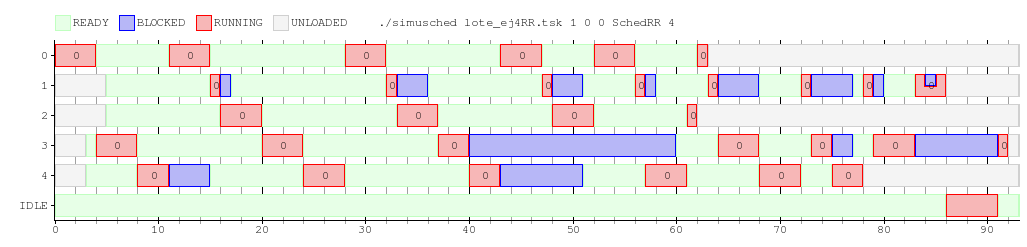
\includegraphics[width=15 cm]{graficos/ej4RR1.png}
\centering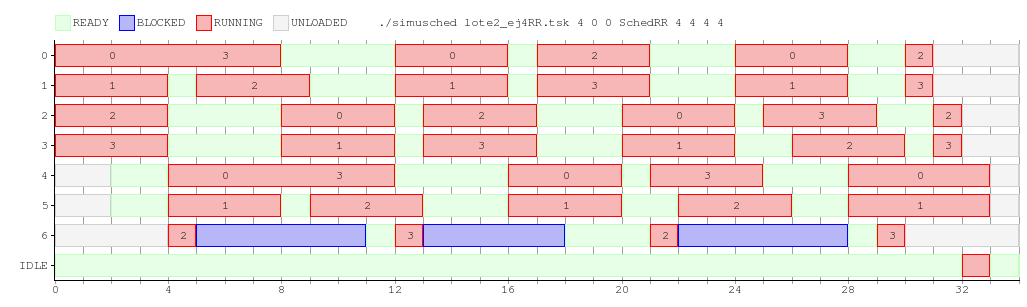
\includegraphics[width=15 cm]{graficos/ej4RR2.png}
\caption{Round-robin, un sólo núcleo de procesamiento en el primer caso, 4 en el segundo. Distintos lotes de tareas.}
\end{figure}

Se confeccionaron dos lotes diferentes para la figura 2. Para el primer caso se corrieron dos TaskCPU, una TaskConsola y dos TaskAlterno (alternan entre uso de CPU y llamadas bloqueantes). Como el primer gráfico muestra el comportamiento con un único núcleo es facil ver como SchedRR funciona. En orden de llegada cada tarea corre su quantum, o lo pierde si se bloquea para que otra tome su lugar.

El segundo caso refleja el mismo funcionamiento pero quad-core, con iguales quantums máximos para cada CPU. En este caso el lote estaba compuesto por seis TaskCPU y sólo una TaskConsola. Como en el ejemplo no hay costos de migración, algunas tareas terminan el quantum de un núcleo y automáticamente corren en otro, pero es de esperarse. La TaskConsola se bloquea y libera el CPU para otras tareas.

\subsection{SchedLottery y compensaciones probabilísticas}

\subsubsection{Idea general}

Las tareas que utilizan I/O (como por ejemplo las interactivas) traen aparejada una desventaja respecto a las de uso de CPU cuando se las analiza en función de la métrica \emph{turn-around} time,
independientemente del scheduler que esté siendo utilizado. Si consideramos 2 tareas distintas: una bloqueante y una de uso intensivo de CPU que necesitan la
misma cantidad de tiempo de procesamiento y cuentan con un core entero a su disposición, las tareas bloqueantes tendrán indefectiblemente un \emph{turn-around} time mayor, debido al tiempo que
permanecen bloqueadas.

\begin{figure}[H]
  \centering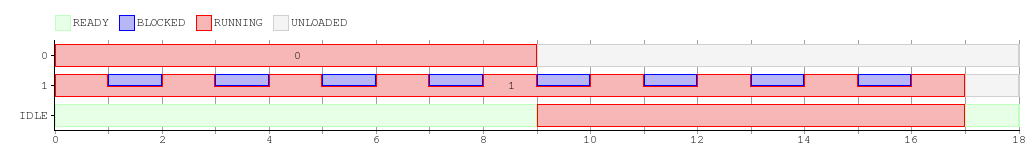
\includegraphics[scale=0.5]{graficos/inherente.png}
  \caption{Procesamiento simultáneo de una tarea I/O y otra de uso\_CPU}
\end{figure}

En el caso mostrado en el gráfico de arriba, ambas tareas requieren de 10 ticks de cpu para finalizar. Sin embargo, la tarea bloqueante tarda el doble de tiempo en terminar. 

En el ejercicio 5 implementamos un scheduler en base al paper ''Lottery scheduling''. El mismo está diseñado para equilibrar esta desigualdad entre el \emph{turn-around} de las tareas relacionado con el
naturaleza de las mismas. El scheduler seleccionea la tarea a la cual será asignado el procesador durante el próximo quantum mediante un sorteo, en donde las probabilidades de ganar
de cada una son inversamente proporcionales a la fracción de quantum que utilizaron la última vez que fueron ganadoras. Para ello se utiliza un sistema de \textbf{tickets}.
Las tareas que consumieron la totalidad del quantum disponen de un único ticket, mientras que las tareas que consumieron una fracción $\frac{f}{q}$ del quantum disponen de $\frac{q}{f}$ tickets (redondeado
hacia arriba). La tarea a la cual se le asignará el procesador durante el próximo quantum será la que tenga el ticket ganador del sorteo entre la totalidad de los mismos.

De esta manera, las tareas de I/O tendrán más probabilidades de ganar los sorteos respecto a aquellas que utilizan la totalidad del CPU. Esto provoca una reducción en el \emph{waiting time} de las mismas 
(ya que deben esperar menos para volver a correr), y por lo tanto también en su \emph{turn-around} time.

\subsubsection{Estructuras auxiliares}

\begin{itemize}
  \item vector<int> cpu\_quantum: Arreglo en donde hay una posición por cada uno de los cores. En cada una queda registro de la cantidad de ticks durante los cuales el procesador ha permanecido
  en posesión del proceso actual. 
  \item semilla: parámetro inicial que determina el inicio de la secuencia pseudoaleatoria. Es muy importante ir variando este valor en el momento de 
  realizar los sorteos, para cambiar la secuencia aleatoria utilizada y simular elecciones aleatorias.
  \item cantTickets: La cantidad de tickets total que participarán en el próximo sorteo.
  \item max\_quantum: Determina la duración del quantum. Sea \emph{core} uno de los procesadores.\\ 
  Cuando cpu\_quantum[core] $\geq$ max\_quantum, la tarea ha consumido la totalidad del quantum y es necesario realizar
  un sorteo para determinar la próxima tarea que será ejecutada.
  \item vector<tarea,\#tickets> tareasReady: Arreglo que contiene las tareas listas para correr, junto con la cantidad de tickets con la que participarán en el sorteo.$\geq$ max\_quantum, la tarea ha consumido la totalidad del quantum y es necesario realizar
  \item vector<tarea,\#tickets> tareasBlocked: Arreglo que contiene las tareas bloqueadas junto con la cantidad de tickets con las que participarán en el sorteo cuando vuelvan al estado Ready
\end{itemize}

\subsubsection{Pseudocódigo}

\begin{algorithmic}
  \Function{load}{int pid}
      \State Agrego a tareasReady la tupla <pid,1>
      \State $cantTickets \gets cantTickets+1$;
  \EndFunction
\end{algorithmic}

~

Al ser cargadas, las tareas comienzan inicialmente con un único ticket. Es importante actualizar la variable \emph{cantTickets} para dejar actualizado el sorteo.

~

\begin{algorithmic}
  \Function{unblock}{int pid}
      \State Agrego a tareasReady la tupla <pid,\#tickets>, (\#tickets está almacenado en tareasBlocked).
      \State Elimino de tareasBlocked la tupla <pid,\#tickets>
      \State $cantTickets \gets cantTickets+\#tickets$;
  \EndFunction
\end{algorithmic}

~

Las tareas recientemente desbloqueadas participarán del próximo sorteo, por lo que son agregadas a \emph{tareasReady} y retiradas de \emph{tareasBlocked}.
Es importante actualizar la variable \emph{cantTickets} para dejar actualizado el sorteo.

~

\begin{algorithmic}
  \Function{tick}{int cpu, Motivo m}
      \State $actual \gets$ tarea que está siendo ejecutada por el \emph{cpu} actualmente
      \State $proximo \gets$ actual
      
      \If{m==EXIT}
	  \State cpu\_quantum[cpu]=0 (Reseteo el quantum)
	  \If{!tareasReady.empty()}
	      \State $proximo \gets lottery()$
	  \Else
	      \State $proximo \gets IDLE\_TASK$
	  \EndIf
      \EndIf
      \State
      \If{m==BLOCK}
	  \State cpu\_quantum[cpu]++ 
	  \State \#tickets = $\frac{max\_quantum}{cpu\_quantum[cpu]}$ 
	  \State
	  \State (La tarea se bloqueó, por lo que no utilizó la totalidad del quantum.
	  \State Se le asigna una cantidad de tickets inversamente proporcional 
	  \State a la fracción de quantum que haya utilizado.)
	  \State
	  \State Agrego a tareasBlocked la tupla <actual,\#tickets>
	  \State cpu\_quantum[cpu] $\gets 0$
	  \If{!tareasReady.empty()}
	      \State $proximo \gets lottery()$
	  \Else
	      \State $proximo \gets IDLE\_TASK$
	  \EndIf
      \EndIf
      \State
      \If{m==TICK}
	  \State cpu\_quantum[cpu]++
	  \If{actual==IDLE\_TASK}
	      \If{!tareasReady.empty()}
		  \State cpu\_quantum[cpu]=0 
		  \State $proximo \gets lottery()$
	      \EndIf
	      \State(Si no hay otras tareas, continúo ejecutando la IDLE)
	  \Else(se está ejecutando una tarea)
	      \If{cpu\_quantum $\geq$ max\_quantum}
		  \If{!tareasReady.empty()}
		      \State cpu\_quantum[cpu]=0 (Reseteo el quantum)
		      \State $proximo \gets lottery()$
		  \EndIf
		  \State(Si no hay otras tareas, continúo ejecutando la misma)
	      \EndIf
	   \EndIf
      \EndIf
  \EndFunction
\end{algorithmic}

~

\begin{algorithmic}
  \Function{lottery}{}
	\State $suma \gets 0$
      	\State $semilla++$
	\State srand(semilla)
	\State $ticketGanador \gets (rand() \% cantTickets)+1$
	\For{$i \gets 0$ to tareasReady.size()}
		\State $suma \gets suma+ \#tickets$ de tarea i		
		\If{$ticketGanador \leq suma$}
			\State $res \gets$ tarea i
			\State $cantTickets \gets $ \#tickets de tarea i	
			\State Borro la tarea i de tareasReady
			\State break
		\EndIf
	\EndFor	
	\State \Return res
  \EndFunction
\end{algorithmic}

~

Para realizar el sorteo se selecciona un número aleatiro utilizando las funciones rand y srand (ya explicadas con anterioridad).

Incrementamos el valor de la semilla para que la próxima vez el sorteo se realice con una secuencia pseudoaleatoria distinta. Esto es muy importante
para lograr la simulación de un sorteo con elecciones aleatorias.

El sorteo se realiza específicamente en la línea: $ticketGanador$ = ( rand() \% (cantTickets) ) + 1.

Recorremos la lista hasta encontrar la tarea con el ticket ganador.

Decrementamos la cantidad de tickets y retiramos $res$ de la lista de tareasReady.

~

\begin{figure}[H]
  \centering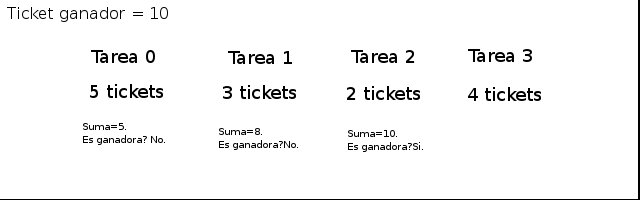
\includegraphics[scale=0.5]{graficos/lottery.jpg}
  \caption{Funcionamiento de lottery()}
\end{figure}

~

\subsubsection{Experimentando con SchedLottery con compensation tickets}

~

\textbf{\underline{Lote TaskCPU}}

Simulemos en primer lugar el comportamiento de nuestro scheduler para un lote de tareas de cálculo: es decir, procesos que no 
efectúan instrucciones de I/0. A lo largo de la ejecución habrá tantos tickets como tareas, cada uno correspondiente a una
tarea distinta. Por lo tanto, dado un lote de $n$ tareas cada una tiene una probabilidad de $\frac{1}{n}$ de obtener el procesador
en el próximo quantum. El comportamiento esperado es de alguna forma similar al de round robin, ya que se espera que cada $n$
quantums, cada tarea haya sido ejecutada durante 1 quantum.


\begin{figure}[H]
  \centering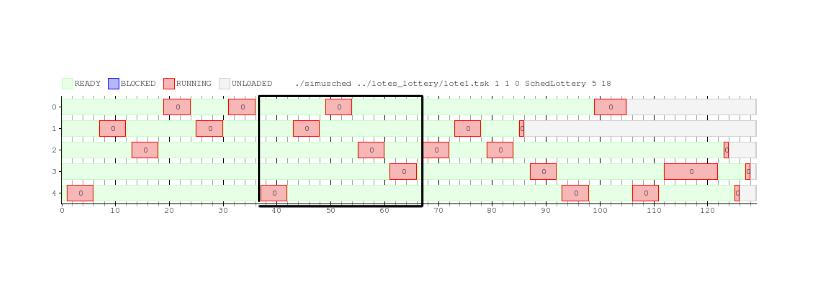
\includegraphics[scale=0.5]{graficos/lottery_cpu.jpg}
  \caption{SchedLottery en un lote de procesamiento cientifico. lote: *5 TaskCPU 20.
	1 core, cambio de contexto = 1, migración = 0, quantum = 5}
\end{figure}

~

Efectivamente, en el recuadro negro que aparece en la figura se observa un comportamiento muy similar al de Round-Robin.

\begin{itemize}
	\item tarea 0: wt:21, ta:105
	\item tarea 1: wt:13, ta:86
	\item tarea 2: wt:20.6, ta:124
	\item tarea 3: wt:26.75, ta:128
	\item tarea 4: wt:21, ta:126
	\item  Waiting time: 20.47
	\item  Turnaround time: 113.8
\end{itemize}


Observemos que tanto el wating time como el turn around time de cada una de las tareas no difiere demasiado entre sí (tal como hubiera sucedido en el Round-Robin).
Si realizamos 20 corridas del mismo experimento, para un único core pero variando el quantum entre 1 y 5, obtenemos los siguientes gráficos, en donde se muestran
el waiting-time promedio y el $turn-around$ promedio.


\begin{figure}
\hfill
\subfigure[]{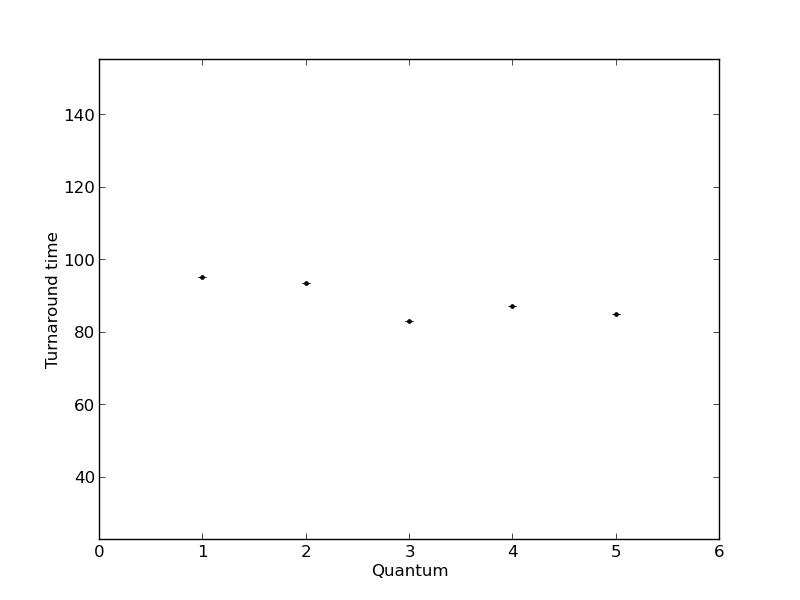
\includegraphics[width=8.75cm]{graficos/lottery_cpu_ta.jpg}}
\hfill
\subfigure[]{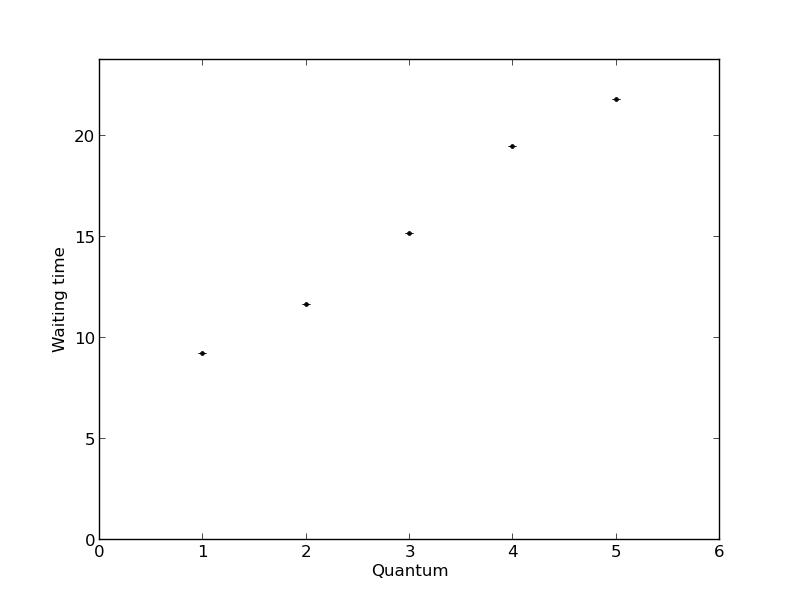
\includegraphics[width=8.75cm]{graficos/lottery_cpu_wt.jpg}}
\hfill
\caption{Turn around time y waiting time del SchedLottery del mismo lote de procesamiento cientìfico con los mismos paràmetros,
	pero variando los quantums entre 1 y 5}
\end{figure}

El waiting-time promedio de 20 repeticiones para 5 cores es de 22, cercano al experimento particular aislado, en donde obtuvimos 20.47.
El turn-time promedio de 20 repeticiones para 5 cores es de 100, cercano al experimento particular aislado, en donde obtuvimos 113.8

~

Si comparamos los resultados obtenidos con los de un scheduler round-robin obtenemos:

\begin{figure}
\hfill
\subfigure[]{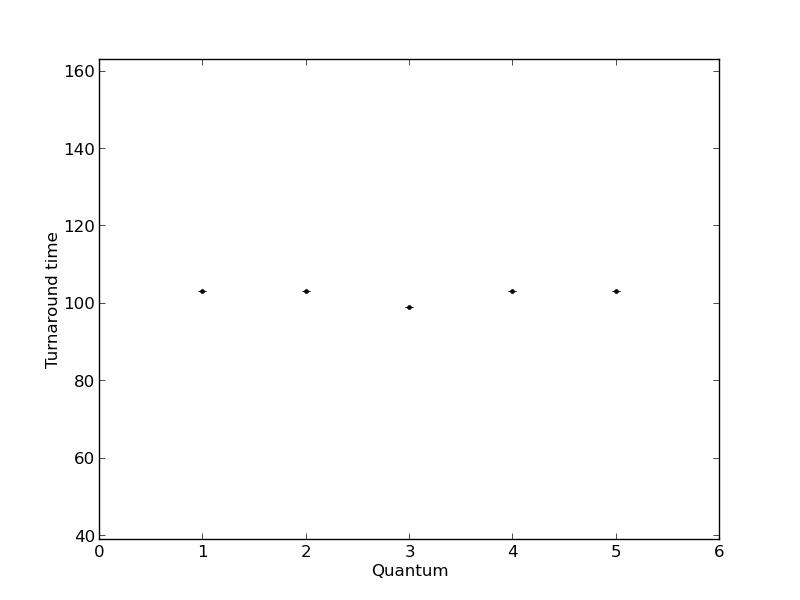
\includegraphics[width=8.75cm]{graficos/lottery_rr_ta.jpg}}
\hfill
\subfigure[]{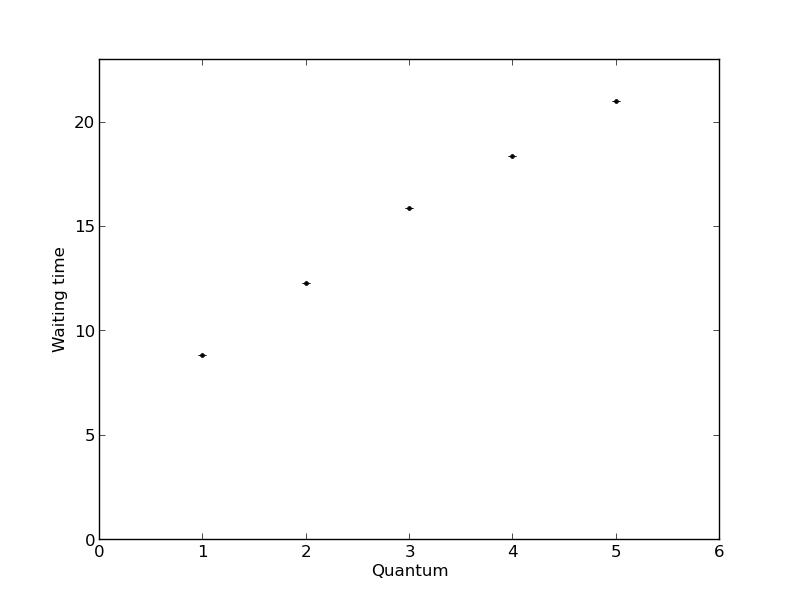
\includegraphics[width=8.75cm]{graficos/lottery_rr_wt.jpg}}
\hfill
\caption{Turn around time y waiting time del Round Robin del mismo lote de procesamiento cientìfico con los mismos parámetros,
	pero variando los quantums entre 1 y 5}
\end{figure}

Tal como era esperable, para lotes con tareas de igual cantidad de tickets ambos schedulers se comportan de forma muy similar.
Sorprende a simple vista lo similares que son los gráficos correspondientes a uno y otro Scheduler, pero realmente corresponden a experimentos distintos.




En el ejercicio 5 implementamos un scheduler en base al paper ''Lottery scheduling''. El mismo está diseñado para equilibrar esta desigualdad entre el \emph{turn-around} de las tareas relacionado con el
Para ejemplificar lo mencionado anteriormente, supongamos que en una computadora de un solo core se han lanzado dos procesos que corren en simultáneo. El primero de ellos, al cual llamaremos $A$, utiliza
activamente el CPU sin necesidad de hacer llamados al sistema o esperar que se liberen recursos de la máquina (podría ser, por ejemplo, el caso de una aplicación científica que ejecuta gran cantidad de 
cuentas). Por otro lado tenemos a la tarea $B$, que ejecuta una instrucción bloqueante cada cierto tiempo, desbloquéandose luego de una cierta cantidad de ticks del reloj. Supongamos también que ambos conviven
con otros procesos que también están siendo ejecutados por el cpu. En el caso de un scheduler Round Robin, a lo largo de una ronda se le asigna un quantum a cada proceso. Sin embargo, notemos que mientras
la tarea $A$ utiliza la totalidad del quantum que le han asignado, $B$ usa únicamente una fracción: $\frac{f}{q}$. De esta manera, luego de sucesivas rondas la tarea $A$ ha sido ejecutada un tiempo
considerablemente mayor al de $B$.

Para solucionar este problema, la idea es que el scheduler seleccione la próxima a ser ejecutada mediante el sorteo de una lotería, en donde aquellas tareas que utilicen solamente una fracción del quantum
tengan más probabilidades de ser las ganadoras. Para lograr este objetivo, utilizamos un sistema de ''compensation tickets'', que funciona de la siguiente manera:

- Las tareas que llegan por primera vez entran con una cantidad equivalente a $\frac{\#tickss}{quantum}$. Por ejemplo, si cada quantum consta de 8 ticks, entonces cada
proceso recibirá 8 tickets iniciales, con lo cual evitamos que las tareas recién ingresadas sufran de inanición (se les dé la oportunidad de correr para conocer su tipo, 
y comepensarlos (o no) con la cantidad de tickets correspondiente).

- Cuando una tarea es desalojada debido a una llamada bloqueante, lo más probable es que solamente haya utilizado una fracción del quantum. Sea esta última $\frac{f}{q}$,
en donde q es igual a $\frac{\#tickss}{quantum}$ y f la cantidad de ticks consumidos por la tarea durante el último llamado.
Anteriormente habíamos dicho que el scheduler debía encargarse de que todas las tareas corrieran una cantidad de tiempo lo más similar posible a las demás, y que para ello utilizaba
el sistema de compensation tickets. Nuestro mecanismo hace que la tarea ingrese a la cola de Ready's con $\frac{q}{f}$ tickets, con lo cual tiene una probabilidad de ganar
inversamente proporcional a la fracción de quantum que está usando.

- Cuando se produce un tick y el scheduler detecta que la tarea consumió la totalidad de su quantum, la misma es desalojada y encolada en el vector de Ready's con un solo ticket.

~


Poniendo en un ejemplo lo anteriormente mencionado, supongamos una máquina con un scheduler con
un quantum de 8 ticks manejando temporalmente 
1 tarea bloqueante $A$ (cuyos bloqueos duran 1 ciclo), y 2 tareas $B$ y $C$ que consumen CPU. En un principio todas entran al sorteo con 8
tickets. Sin embargo, luego de que las tres han corrido por lo menos una vez, siempre entrarán al sorteo con una misma cantidad: $A=8, \ B=1, \ C=1$, con un total de
10 tickets en circulación. Con estos valores, se espera que cada 10 sorteos (número que coincide con la cantidad de tickets en circulación): 8 sean ganados por A,
1 sea ganado por B y 1 por C, con lo cual todas estarían corriendo la misma cantidad de ticks en el cpu. 

~

\textbf{\underline{Lote TaskConsola, igual cantidad de tickets}}

Simulemos ahora el comportamiento de nuestro scheduler para un lote de tareas interactivas: por ejemplo, TaskConsola.
Consideremos para una primera etapa un lote en donde las tareas se bloqueen la misma cantidad de ticks de CPU. Se espera que suceda algo muy similar
al experimento anterior. El scheduler debería tener un comportamiento similar al de Round-Robin, ya que las tareas tendrían la misma cantidad de tickets
en cada sorteo.
 
\begin{figure}[H]
  \centering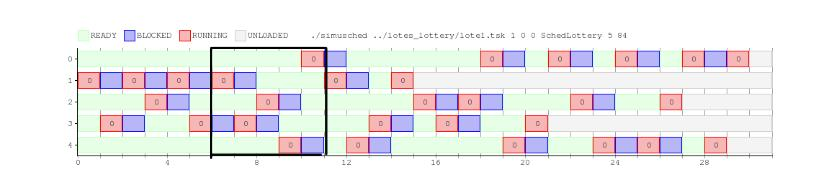
\includegraphics[scale=0.5]{graficos/lottery_console.jpg}
  \caption{SchedLottery en un lote de tareas interactivas. lote: *5 TaskConsola 5 1 1.
	1 core, cambio de contexto = 1 y migración = 0, quantum = 5}
\end{figure}
 
Efectivamente, en el recuadro negro que aparece en la figura se observa un comportamiento muy similar al de Round-Robin.

\begin{itemize}
  \item tarea 0: wt:8.16667, ta:60
  \item tarea 1: wt:3.16667, ta:30
  \item tarea 2: wt:7.16667, ta:54
  \item tarea 3: wt:5.16667, ta:42
  \item tarea 4: wt:7.83333, ta:58
  \item Waiting time promedio: 6.3
  \item Turnaround time promedio: 48.8
\end{itemize}

En esta corrida en particular el desvío estandar de ambas métricas es bastante grande, aunque interviene mucho el factor pseudoaleatorio.
Al repetir el experimento 20 veces con los mismos parámetros, variando los quantums entre 1 y 5 obtenemos:


\begin{figure}
\hfill
\subfigure[]{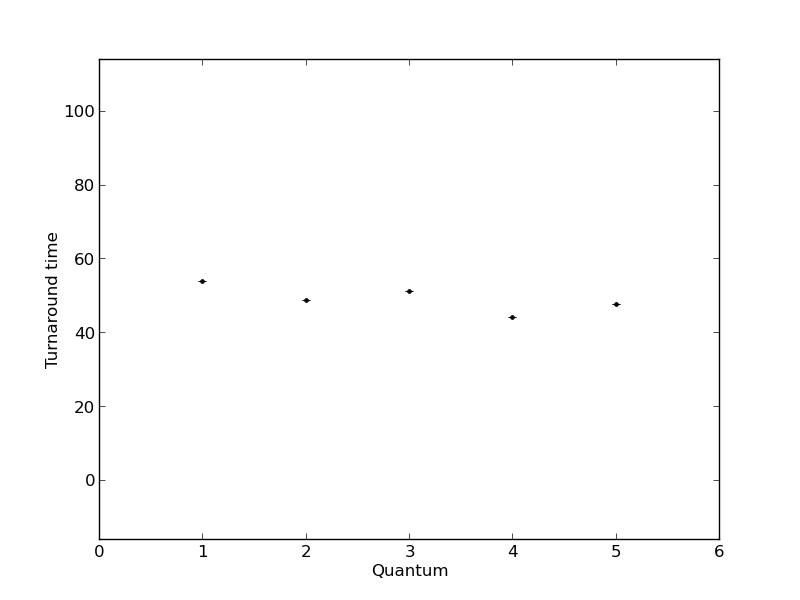
\includegraphics[width=8.75cm]{graficos/lottery_console_ta.jpg}}
\hfill
\subfigure[]{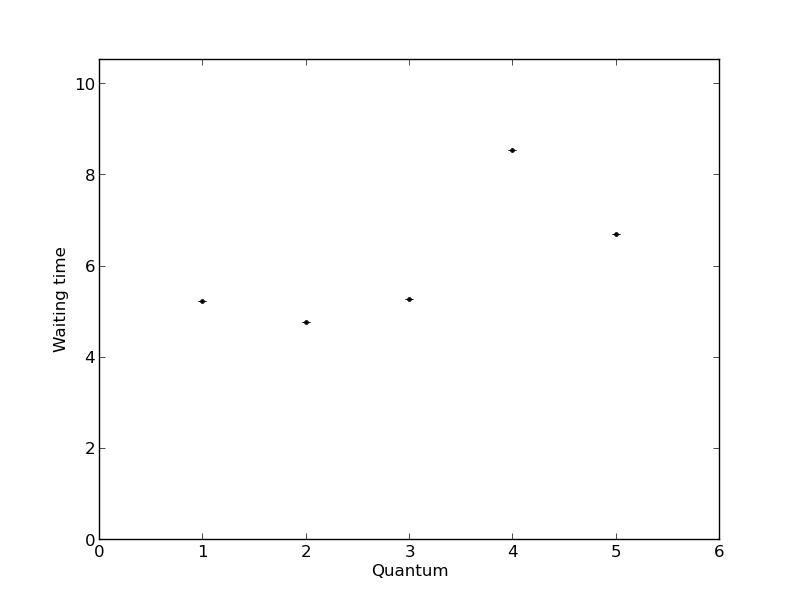
\includegraphics[width=8.75cm]{graficos/lottery_console_wt.jpg}}
\hfill
\caption{Turn around time y waiting time del SchedLottery del lote de procesamiento interactivo con los mismos parámetros,
	pero variando los quantums entre 1 y 5}
\end{figure}

Comparando con el Round-Robin para el mismo lote, nuevamente obtenemos valores muy similares. El mismo comportamiento analizado en el lote CPU puede
observarse tambien en el lote interactivo, para tareas que se bloquean la misma cantidad de ticks.

\begin{figure}
\hfill
\subfigure[]{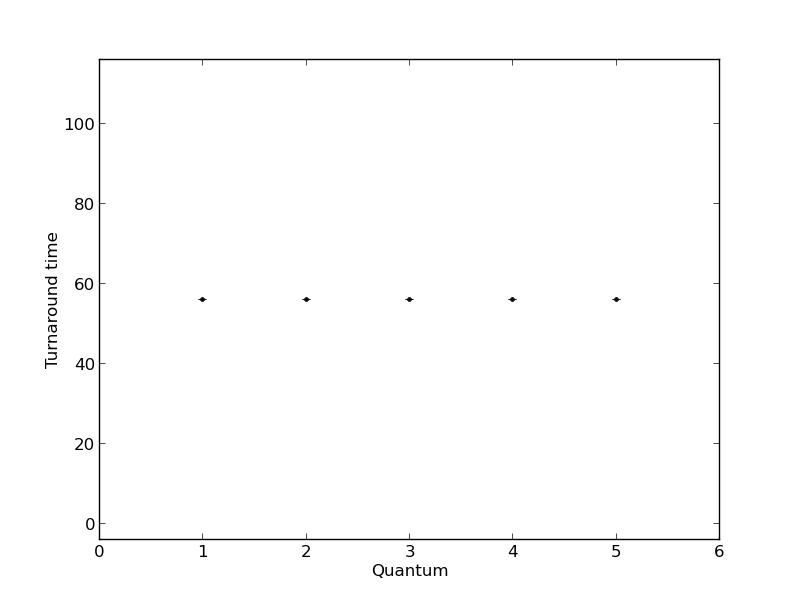
\includegraphics[width=8.75cm]{graficos/console_rr_ta.jpg}}
\hfill
\subfigure[]{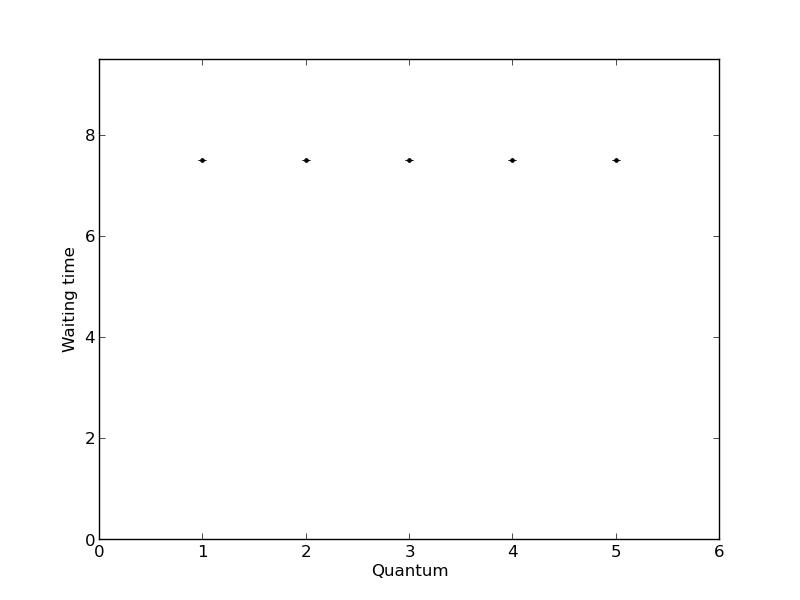
\includegraphics[width=8.75cm]{graficos/console_rr_wt.jpg}}
\hfill
\caption{Turn around time y waiting time del RoundRobin del lote de procesamiento interactivo con los mismos parámetros,
	pero variando los quantums entre 1 y 5}
\end{figure}

~

\textbf{\underline{Lote variado: Apreciación de los compensation tickets}}

Los lotes en donde nos damos cuenta de la diferencia que marcan los compensation tickets es en aquellos que son mixtos. Combinan tareas bloqueantes con no
bloqueantes, por lo que estas últimas deberían tener más tickets y por lo tanto, ganar más sorteos y reducir el turn around time.

\begin{figure}[H]
  \centering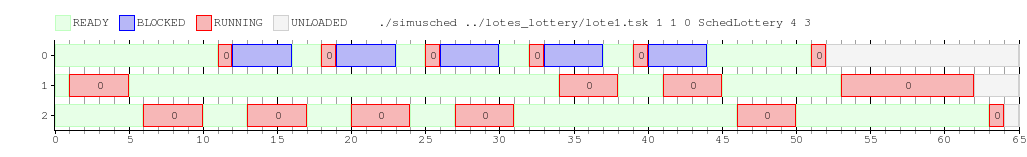
\includegraphics[scale=0.5]{graficos/mixto.png}
  \caption{SchedLottery en un lote de tareas mixto. lote: TaskConsola 5 4 4, *2 TaskCPU 20.
	1 core, cambio de contexto = 1 y migración = 0, quantum = 4}
\end{figure}

\begin{itemize}
	\item tarea bloqueante: wt:7.5, ta:51
	\item tarea cpu: wt:7.8, ta:65
	\item tarea cpu: wt:8, ta:61
	\item  Waiting time: 7.76667
	\item  Turnaround time: 59
\end{itemize}

Hay que destacar que la tarea bloqueante gana muchos más sorteos que las otras dos tareas de procesamiento, ya que dispone de 4 tickets (las otras 2 cuentan con 1 único tickets).
No es casualidad que la tarea bloqueante disponga del waiting time más bajo de todas.

~

\textbf{\underline{Sin la optimización de compensation tickets}}

Sin las optimizaciones, tal como mencionamos anteriormente, el scheduler se comporta muy similar a un round robin, ya que todas tienen las mismas probabilidades de salir sorteadas.


\subsubsection{Ecuanimidad del SchedLottery}

En el ejercicio 5 implementamos un scheduler en base al paper ''Lottery scheduling''. Intentamos generar un mecanismo de control eficiente, flexible y justo en donde cada tarea fuese procesada
aproximadamente un tiempo equivalente a las otras, sin importar su tipo. Este último aspecto es el que nos permite hablar de ecuanimidad del scheduler.

Para ejemplificar lo mencionado anteriormente, supongamos que en una computadora de un solo core se han lanzado dos procesos que corren en simultáneo. El primero de ellos, al cual llamaremos $A$, utiliza
activamente el CPU sin necesidad de hacer llamados al sistema o esperar que se liberen recursos de la máquina (podría ser, por ejemplo, el caso de una aplicación científica que ejecuta gran cantidad de 
cuentas). Por otro lado tenemos a la tarea $B$, que ejecuta una instrucción bloqueante cada cierto tiempo, desbloquéandose luego de una cierta cantidad de ticks del reloj. Supongamos también que ambos conviven
con otros procesos que también están siendo ejecutados por el cpu. En el caso de un scheduler Round Robin, a lo largo de una ronda se le asigna un quantum a cada proceso. Sin embargo, notemos que mientras
la tarea $A$ utiliza la totalidad del quantum que le han asignado, $B$ usa únicamente una fracción: $\frac{f}{q}$. De esta manera, luego de sucesivas rondas la tarea $A$ ha sido ejecutada un tiempo
considerablemente mayor al de $B$.

Para solucionar este problema, la idea es que el scheduler seleccione la próxima a ser ejecutada mediante el sorteo de una lotería, en donde aquellas tareas que utilicen solamente una fracción del quantum
tengan más probabilidades de ser las ganadoras. Para lograr este objetivo, utilizamos un sistema de ''compensation tickets'', que funciona de la siguiente manera:

- Las tareas que llegan por primera vez entran con una cantidad equivalente a $\frac{tickets}{1 \ quantum}$. Por ejemplo, si el 
- Las tareas que utilizaron la totalidad del quantum la último





 

%\subsection{Experimentos}

Para verificar el $fairness$ de nuestro scheduler decidimos cargarle una determinada cantidad de tareas y comparar cuántos ticks insumía cada una en un rango determinado. Si efectivamente existe ecuanimidad, cada una de las tareas debería insumir una cantidad similar de ticks.

Para testear este comportamiento tomamos el siguiente lote de tareas: una bloqueante y tres que consumen cpu. Las tres insumen en total una cantidad fija de cilos. La bloqueante bloquea 16 veces y las demás tienen un quantum de 32. Como se trata de un scheduler $pseudoaleatorio$ fue necesario realizar el expermimento varias veces con el objetivo de evitar resultados indeseados.

Decidimos tomar como rango inicial el instante en el que todas las tareas ya fueron ejecutadas ya que a partir de allí comenzarán a influir los $compensations \ tickets$. El rango final se determinó de forma arbitraria cersiorándose de que se encuentre antes de la finalización de alguna tarea.

Realizamos el experimento para un scheduler de 1 core y un quantum de 4 y los resultados fueron los siguientes:

\begin{figure}[!h]
	\begin{center}
		  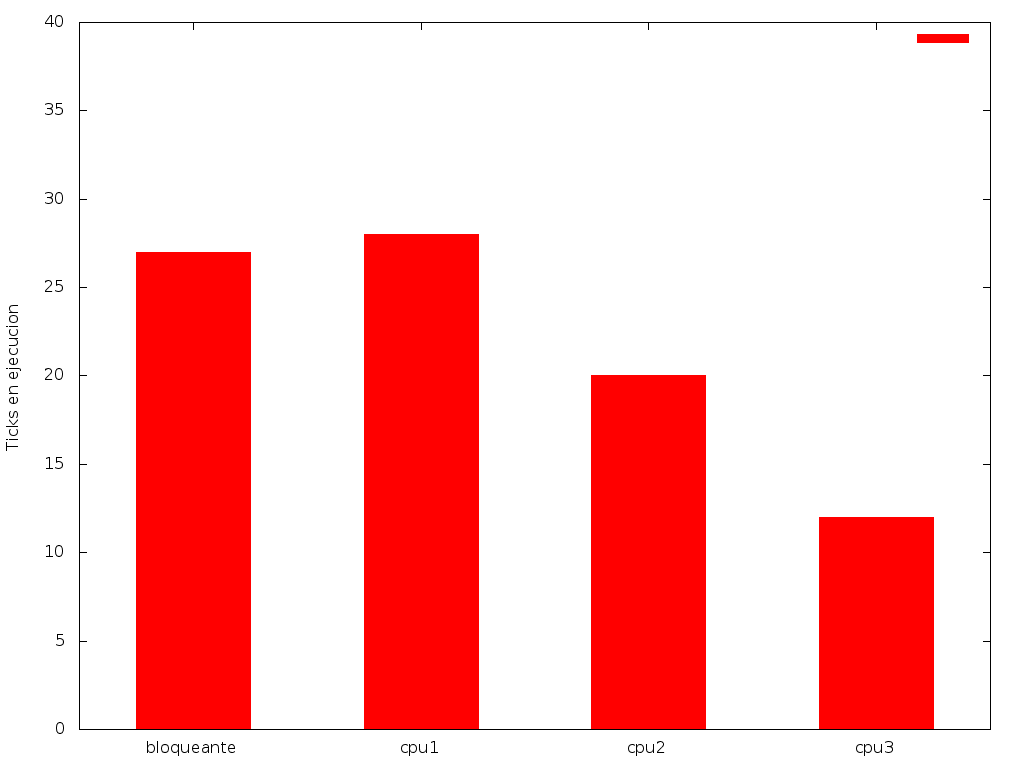
\includegraphics[scale=0.3]{Graficos/comp1.png}
		  \caption{Ticks insumidos por cada tarea para un schedLottery de 4 tareas: 1 bloqueante y 3 de CPU (1 core)}
		  \label{fig:contra1}
	\end{center}
\end{figure}
\FloatBarrier

Para 2 cores ocurrió lo siguiente:

\begin{figure}[!h]
	\begin{center}
		  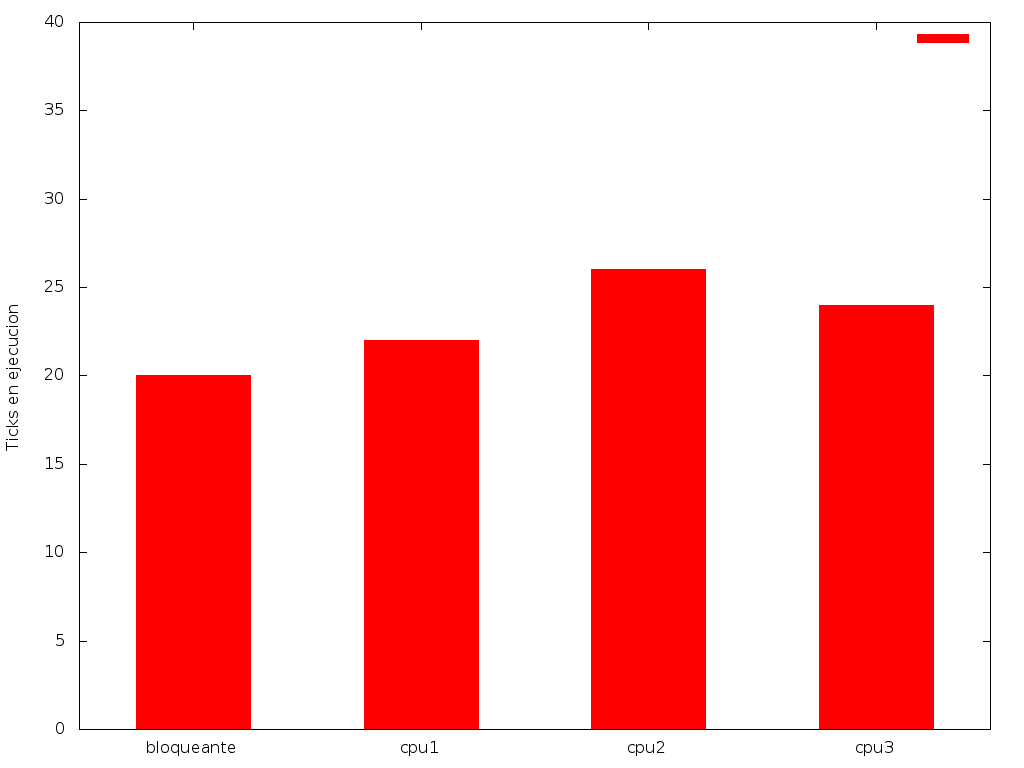
\includegraphics[scale=0.3]{Graficos/comp2.png}
		  \caption{Ticks insumidos por cada tarea para un schedLottery de 4 tareas: 1 bloqueante y 3 de CPU (2 core) }
		  \label{fig:contra1}
	\end{center}
\end{figure}
\FloatBarrier

Como se puede observar, los ticks insumidos por cada tarea es bastante equitativa. Esto quiere decir que los $compensation \ tickets$ están actuando a favor de la tarea bloqueante que es la que utiliza solo una parte de su quantum cada vez que se ejecuta.

Los $compensation \ tickets$ son los que lo otorgan equanimidad a este scheduler. Sin ellos la tarea bloqueante no hubiera insumido los ticks que insumió en las pruebas anteriores. Para comprobar esto, corrimos el mismo scheduler con el mismo lote de tareas pero sin $compensation \ tickets$. Estos fueron los resultados:

Para 1 core:

\begin{figure}[!h]
	\begin{center}
		  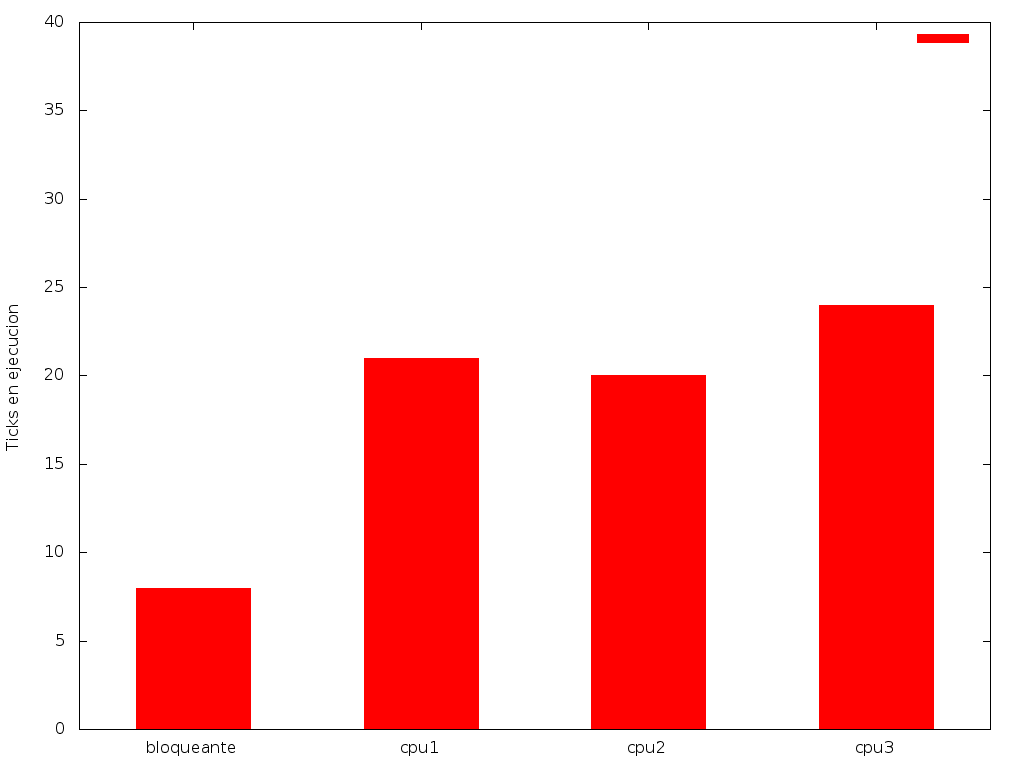
\includegraphics[scale=0.3]{Graficos/sincomp1.png}
		  \caption{Ticks insumidos por cada tarea para un schedLottery de 4 tareas: 1 bloqueante y 3 de CPU (1 core). Sin $compensation \ tickets$}
		  \label{fig:contra1}
	\end{center}
\end{figure}
\FloatBarrier

Para 2 cores:

\begin{figure}[!h]
	\begin{center}
		  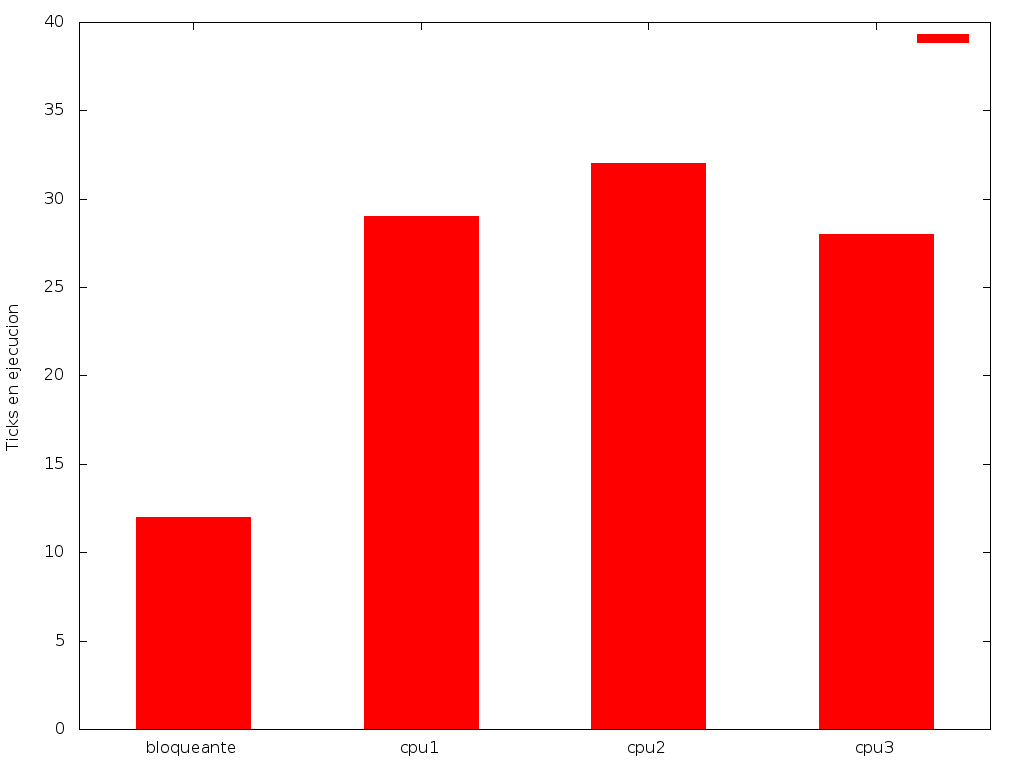
\includegraphics[scale=0.3]{Graficos/sinComp2.png}
		  \caption{Ticks insumidos por cada tarea para un schedLottery de 4 tareas: 1 bloqueante y 3 de CPU (1 core). Sin $compensation \ tickets$}
		  \label{fig:contra1}
	\end{center}
\end{figure}
\FloatBarrier

Como puede oservarse, los ticks insumidos por la tarea bloqueante es mucho menor de lo que era antes. La ecuanimidad ya no está presente en este scheduler.

